\section{Feature / Label Agreement}

\subsection{Useful Features for Classification}
In the next section we detail which features will be useful for future tasks and which will not. We were careful not to preemptively bias ourselves against using certain features simply because they do not seem useful with the analysis we have performed so far.
\subsubsection{Methodology:}

\begin{enumerate}
    \item \textbf{Analysing feature variance}: We looked at each feature and applied simple metrics to them such as computing mean, median and standard deviation values. The resulting processed dataset allows us to quickly eliminate features we deem to be too unstable to train a reliable classifier on.
    \item \textbf{Correlation Analysis}: Additionally, we looked at the uniqueness of each feature to see which ones are the most sensitive to subtle differences in the source data.
\end{enumerate}

\subsubsection{Findings:}

\begin{itemize}
    \item \textbf{1D features}: At first glance, we identified the bandwidth, centroid, YIN and zero crossing rate (ZCR) 1D features as quite sensitive to the input data with each one producing a fairly unique pattern over time. The former and latter two are mostly quite similar, though we ultimately prefer the centroid and ZCR features for being more stable and more descriptive of the input pattern, especially for similar words.
    \item \textbf{2D features}: Out of the 2D features available, we found the mel spectrogram to be the most promising one due to the amount of data available. We believe that he MFCC features while smaller would still be a good enough choice to include into a classifier.
    \item \textbf{Model Implications}: We come to the conclusion that not all of the features will be required to train a classifier which will ease the resource constraints of the final system considering that the target platform are low power embedded devices.
\end{itemize}

\begin{figure}[!ht]
	\centering
	\begin{minipage}{0.49\textwidth}
		\centering
		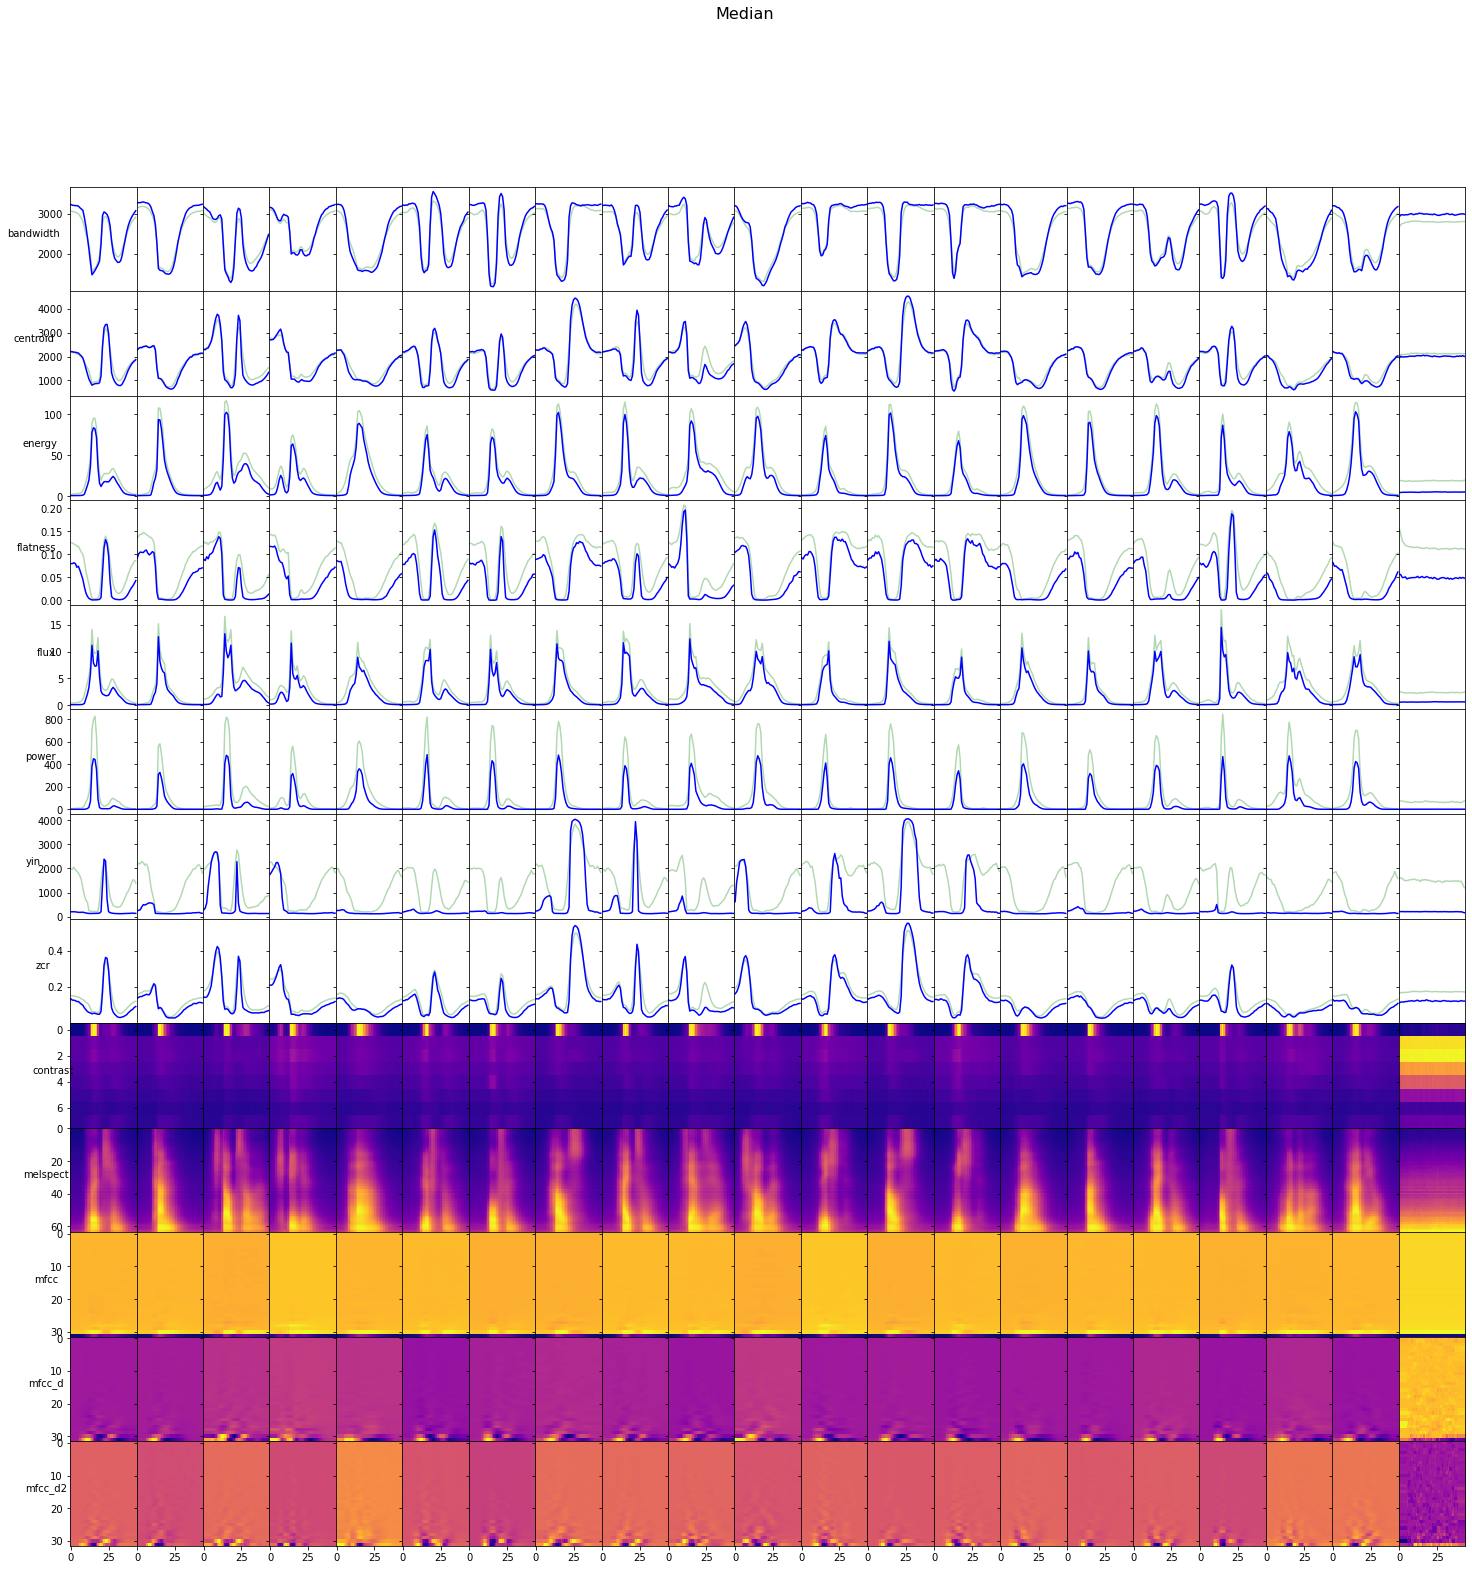
\includegraphics[scale=0.3]{fig/Task2.4_Summary.png}
		\caption{Overview of the expected features in the dataset.}
		\label{fig:FeaturesSummary}
	\end{minipage}\hfill
\end{figure}

\subsection{Feature Distribution for Similar Words}

Some of the input words are very similar, especially the pair "Licht" and "nicht". The classifier will have to deal with very subtle differences in its input data and overfitting might quickly become a problem.

\subsubsection{Methodology:}

\begin{enumerate}
    \item \textbf{Comparative Analysis}: We compared the features visually and statistically to determine which features are the most sensitive to the subtle changes in the input data.
\end{enumerate}

\subsubsection{Findings:}

\begin{itemize}
    \item \textbf{Feature seperation}: We found that most features, even the ones selected above only yield very poor seperation between the most challenging pairs. The higher order derivatives of the DCT coefficients tend to give the most seperation.
    \item \textbf{Implications for the classifier}: We must therefore conclude that any future classifier will have to be trained for very subtle differences and perhaps be context sensitive in order to reliably detect very similar words.
\end{itemize}
